
\section{Introducing Formal Languages}

So far, we have been discussing English sentences using English. One of the
great strengths of natural languages is their expressive power and versatility
that enable us to talk about a language using that very language. However, the
long history of the study of logic, languages, and our reasoning abilities shows
that this versatility is also a source of confusion and avoidable errors.
 Systematic treatment is easier if we introduce an artificial language and talk 
 about the features of that language. 

The language that we talk about is the \emph{object language}. The
language we use to talk about the object language is the \emph{meta-language}.  
So far, our object language has been the same language as the meta-language: we 
have been using English to talk about English sentences.  We will change the 
object language to a new artificial language.  Our meta-language remains 
English---no need to learn a new language to continue reading---but the object 
language will be an artificial language whose features we stipulate to suit our 
needs and can control with great precision. The aim is to construct an 
artificial language that can do everything, or nearly everything, by way of 
expressing logical relations that we can in English. But, unlike English, our 
artificial language is incapable of doing much else.

Let us start. Let us call our artificial language \lL[S]{}  (that's a cursive `L' 
as in `language' with a subscript `S' as in `simple').  \lL[S]{} has two 
expressions, $A$ and $B$, that both express sentences.  The following tables 
tell us what they mean:

\begin{center}
 \showttwide{tc-A}
 \showttwide{tc-B}
\end{center}

These tables state the truth conditions of $A$ and $B$. As you can see, when 
a speaker of \lL[S]{} uses $A$ to say something, what they say is true if snow is 
white, and what they say is false otherwise. If the speaker uses $B$ to say 
something, what they say is true if the moon is made of cheese, and what they 
say is false  otherwise. So you could translate $A$ into the English sentence 
`snow is white' and translate $B$ into `the moon is made of cheese'. 

Here is something \emph{very} important to keep in mind. If what I have told you 
about \lL[S]{} exhausts the features of \lL[S]{}, a monolingual speaker of \lL[S]{} 
could not say what I just said in the previous paragraph. In order to say what I 
just said I needed many more sentences than just $A$ and $B$ or their English 
translations. \lL[S]{} does not have any of those sentences available.

For the same reason, a monolingual speaker of \lL[S]{} could not give us the table 
describing when $A$ and $B$ are true. We are using English as our meta-language 
and I am relying on your knowledge of English even if it is not your first 
language.  Because English is so much more powerful than \lL[S]{}, we can describe 
features of \lL[S]{} in ways that native monolingual speakers of \lL[S]{} could not.

So far, \lL[S]{} is not a very useful language. Let us expand it a bit. We want it to 
be able to form compound sentences. To that end, we will introduce the following 
three symbols: \p{\lnot}, \p{\land}, \p{\lor}. Additionally, we also have 
brackets: \p{(} and \p{)}.  These symbols can be used to form the following 
compound sentences:

\begin{slist}

 \item \p{\lnot A}

 \item \p{(A \land B)}

 \item \p{(A \lor B)}
 
\end{slist}

These are the only compound sentences you can form in \lL[S]{} so far. What do 
these sentences express? We can specify that by stipulating the truth conditions 
of these compound sentences. Let's do this one by one. Here is the first.

\begin{center}

 \showttwide{tc-lnot-long}

\end{center}

This tells us that \p{\lnot A} is true iff. $A$ is false: it does not matter 
whether or not $B$ is true. Since we know from above that $A$ is false iff. it 
is not the case that snow is white, \p{\lnot A} is true iff. it is not the case 
that snow is white. So, \p{\lnot A} is the denial of $A$. You could translate 
\p{\lnot A} as `it is not the case that snow is white'. Let us call the \p{\lnot} 
symbol the \emph{negation} sign. 


Let us move to the next compound sentence, \p{(A \land B)}. Its truth condition 
is given by:

\begin{center}

 \showttwide{tc-land}

\end{center}

As you can see,  the compound sentence \p{(A \land B)} is true if and only if 
$A$ and $B$ are both true. So one way of translating \p{(A \land B)} into 
English would be `A and B' (i.e., `snow is white and the moon is made of  
cheese').  Let us call the \p{\land} sign the \emph{conjunction} sign. The 
sentences flanking the sign are called \emph{conjuncts}.

Here is the last compound sentence: \p{(A \lor B)}:

\begin{center}

 \showttwide{tc-lor}

\end{center}

So \p{(A \lor B)} is true if and only if at least one of $A$ or $B$ is true.  
Let us call the \p{\lor} sign the \emph{disjunction} sign. The sentences 
flanking the sign are called  \emph{disjuncts}.

We now have expanded \lL[S]{} to be able to form a few compound sentences. You 
might have noticed that they work an awful lot like the logical connectives 
\pq{it is not the case that}, \pq{and}, and \pq{or} of the English language that 
we discussed in the previous chapter. But they are not quite the same as those 
logical connectives of English yet.

Notice, for instance, that given the specifications so far, a monolingual 
speaker can deny $A$ in their language but cannot deny $B$---the list of 
compound sentences of \lL[S]{} above does not contain one for denying $B$. Nor is 
it yet possible to deny the conjunction \p{(A \land B)}. So we need a bit more 
work to have a useful language.



\section{Truth Tables}

We noted above that \lL[S]{} does not have the ability to express the denial of 
\p{B} even though it can deny \p{A} by the compound sentence \p{\lnot A}. It is 
natural to introduce a way of denying \p{B} by allowing another compound 
sentence: \p{\lnot B}. But notice that merely allowing that \p{\lnot B} is a 
compound sentence of \lL[S]{} does not ensure that it is the denial of \p{B}. We 
could have a language in which a prefix like \p{\lnot} functions differently 
depending on what it is attached to---think of the prefix `ex' used in English; 
sometimes it means something like `outside', other times it means something like 
`previous'.  So just as we stipulated the truth conditions of \p{\lnot A}, we 
need to stipulate the truth conditions for \p{\lnot B}. That's not too difficult: 
take the above table for \p{\lnot A} and replace each \p{A} with \p{B}. But 
there is a problem.  We want to be able to deny any arbitrary sentence. If we 
had to state the truth conditions for each and every sentence, that will get old 
very quickly, and we could not finish the task since there are infinitely many 
possible compound sentences: e.g., we want to be able to deny a denial, deny the 
denial of a denial, etc. We need a concise way of stating the truth conditions 
for the infinitely many possible sentences we could form by prefixing them with 
the negation sign.

Let us not forget that \lL[S]{} is our own creation and we get to control how it 
works. So let us just say that prefixing any sentence of \lL[S]{} with the 
\p{\lnot} sign results in a compound sentence which is the negation of the 
first.  We can represent this using the following table:

\begin{center}
\showttwide{tt-lnot}
\end{center}

This is called the \emph{truth table} for negation. Notice the lower case \p{s}.  
It does not stand for any particular sentence.  Rather, it is a sentence 
\emph{variable} into which you can substitute any sentence of \lL[S]{}. So the 
table is like a template: you can see how the truth value of  the sentence 
\p{\lnot A} depends on the truth value of \p{A} by substituting \p{A} for \p{s} 
everywhere in the above table.  And you can  see how the truth value of the 
sentence \p{\lnot B} depends on the truth value of \p{B} by substituting \p{B} 
into \p{s} everywhere in the table. That is, the truth table for negation  can 
help you figure out the truth conditions for sentences like \p{\lnot A} and 
\p{\lnot B}.  Similarly, if you want to see how the truth value of \p{\lnot (A 
\land B)} depends on the truth value of \p{(A \land B)}, substitute \p{(A \land 
B)} for \p{s} everywhere, like this: 

\begin{center}
 \showttwide{tc-Nab}
\end{center}
 
Notice that this table does not give us the full list of interpretations: given two 
atomic sentence \p{A} and \p{B}, there must be four interpretations. We will look at 
expanding this to a full specification of the truth condition of \p{\lnot(A 
\land B)} that covers all interpretations in the exercises.

A \emph{truth table} tells us how a particular connective like \p{\lnot} works 
by giving us a template for generating tables that tell us how the truth values 
of a complex sentence using that connective depend on the truth values of its 
component sentences.
I have just used the word  `connective' as in `logical connective'.  After all, 
given the truth table, the \p{\lnot} sign in \lL[S]{} works just like the 
English \pq{it is not the case that}: it can be prefixed to any sentence to form 
a denial of that sentence, and the truth value of the resulting sentence is a 
function of the truth value of the original sentence.

Let us now move to the other two connectives. Here is the truth table for 
conjunction:

\begin{center}
 \showttwide{tt-land}
\end{center}

Because a conjunction takes two sentences to form a new one, we indicate that by 
the subscripts 1 and 2.   The subscripts help you keep track of what you 
substitute into what: all occurrences of \p{s_1} must be substituted by the same 
sentence, and ditto for \p{s_2}. But this does \emph{not} mean that you are not 
allowed to substitute the same sentence into both \p{s_1} and \p{s_2}.  

Substituting \p{A} into \p{s_1} and \p{B} into \p{s_2} tells us how the value of 
\p{A \land B} depends on the truth values of \p{A} and \p{B}, and the result of 
the substitution is identical to the truth conditions of \pq{A and B}  that we 
stated previously.  But the truth table also tells us a lot more.  Given any two 
sentences, the table tells us how the truth value of the compound sentence 
generated by connecting the two with the \p{\land} sign depends on the truth 
values of the two component sentences.  

Finally, here is the truth table for disjunction:

\begin{center}
 \showttwide{tt-lor}
\end{center}

We now have everything we need to figure out the truth-conditions for any 
sentence of the forms: \p{\lnot s}, \p{(s_1 \land s_2)}, \p{(s_1 \lor s_2)}.  
The sentences \p{s}, \p{s_1}, \p{s_2} can all be compound sentences themselves.  
What about something you get by prefixing the \p{\land} sign to a sentence, like 
\p{(\land A)}? Well, \lL[S]{} is our creation so let us declare that there are 
no grammatically correct sentences in \lL[S]{} apart from the atomic sentences 
\p{A} and \p{B} and the three types of compound sentences dealt with by the 
three truth tables. Instead of calling these sentences grammatically correct,
logicians call them  \emph{well-formed formulas (wff)}.

Let me remind you that the characterizations of \lL[S]{} that we are giving are all 
given in the meta-language (English, in the current case). A monolingual speaker 
of \lL[S]{} (even the expanded version) could not give the characterizations we have 
just been giving since \lL[S]{} itself does not have the tools that we are using 
in giving the characterizations. Native speakers of a language often have 
trouble spelling out the workings of their own language---mono-lingual speakers 
of \lL[S]{} are an extreme version of that.

Going forward, in reading sentences of \lL[S]{}, you can pronounce  the symbols 
\p{\lnot}, \p{\lor}, and \p{\land} as `not', `or', and `and' just because it 
makes life easier. But keep in mind that those symbols are expressions of \lL[S]{} 
and not words of English. We assign sounds to them for convenience. If your 
native tongue is not English, you might very well prefer to assign different 
sounds. It does not matter so long as we are clear how \lL[S]{} works and that is 
given by their truth tables just discussed.

\remarkbox{

 Those of you familiar with the mathematical concept of function will notice 
 that a truth table represents a function mapping ordered n-tuples of truth 
 values on the left side of the vertical line onto truth values on the right 
 side. That is why the particular kind of connectives we have been interested in 
 are called `truth-\emph{functional}.'
}





\section{The Language of Sentential Logic}{\label{sec:sentential logic}}



So far, our language \lL[S]{} has had only two atomic sentences. That made reasoning 
about them easy but it is also extremely limiting: there are at most 16 
different things we can say about the world using truth-functional compound 
sentences in a language with only two atomic sentences. Let us therefore allow 
many more atomic sentences.  Let us define:


\begin{description}
\item[Definition.]  A formal language \lL{}{} of sentential logic has the 
 following features:
\begin{enumerate}

 \item There are countably many \emph{atomic} sentences.

 \item If \p{s} is a sentence of \lL{}, so is \p{\lnot s}.

 \item If \p{s_1} and \p{s_2} are sentences of \lL{}, so is \p{(s_1 \land 
  s_2)}.

 \item If \p{s_1} and \p{s_2} are sentences of \lL{}, so is \p{(s_1 \lor 
  s_2)}.

 \item There are no other sentences of \lL{}.

 \item Each atomic sentence has a truth value (either true or false).

 \item Given any sentence \p{s} of \lL{},  \p{\lnot s} is true iff. \p{s} is 
  false.

 \item Given any sentences \p{s_1} and \p{s_2} of \lL{}, \p{(s_1 \land s_2)} is 
  true iff. \p{s_1} and \p{s_2} are both true.

 \item Given any sentences \p{s_1} and \p{s_2} of \lL{}, \p{(s_1 \lor s_2)} is 
  true iff. at least one of \p{s_1} and \p{s_2} is true.


\end{enumerate}
\end{description}
That's it. A few remarks:

To say that \lL{} has countably many atomic sentences is to say that you can count 
the atomic sentences in the usual ways (the first, the second, etc.) all the way 
up to infinity. That is, there could be as many atomic sentences as there are 
natural numbers (or positive integers). But no more.

You may have noticed the use of the indefinite article in the definition: 
`\emph{a} formal language \lL{} \ldots'. The above definition does not define any 
particular language. Rather, it states the conditions something must satisfy to 
count as a formal language of sentential logic. There can be many different 
formal languages that fit the bill. They can differ in the number of atomic 
sentences and the meanings of them. For example, \lL[S]{} is a formal language as 
defined here. It just has two atomic sentences. 

The first five conditions specify the \emph{syntax} of \lL{}, the others the 
\emph{semantics}. The syntax tells us  how the sentences of \lL{} look, the 
semantics tells us about the meanings of the sentences.

A sentence as defined above is often called a \emph{well-formed formula (wff)}. 






Notice how compound sentences are built. There are three ways a compound 
sentence can be formed:

\begin{enumerate}
 \renewcommand{\labelenumi}{\roman{enumi}.}

\item prefix a sentence with the negation sign;

\item connect two sentences with the conjunction sign;

\item connect two sentences with the disjunction sign.

 \end{enumerate}

Since these are the only ways, any compound sentence must either be a negation 
of another, a conjunction of two sentences, or a disjunction of two sentences.  
We will say that in the first case the \emph{main connective} is negation, in 
the second case the main connective is conjunction, and in the last case the 
main connective  is disjunction.  The main connective tells you what the last 
step of construction was to get to the compound sentence starting from atomic 
sentences.

The use of brackets is mandatory as given by the definitions.  However, to 
improve readability, you are allowed to do the following:

\begin{itemize}

 \item  If the very first symbol of a sentence is the opening bracket and its 
  matching closing bracket is the very last symbol of the sentence, you may omit 
  that particular pair of brackets.  
 
 \item you may vary them in size as well as shape (e.g., you might use square 
  brackets, curly brackets, etc.) so long as you match both the size and shape 
  of  opening and closing brackets. 

\end{itemize}


Thus, for example, you may write


\begin{center}

 \plsh{KAPKQRW}

\end{center}

instead of 

\begin{center}

 \p{\big(\lbh{-m=false -pretty=false -f KAPKQRW}\big)}

\end{center}


But you may \emph{not} write \p{\lnot A \land B} instead of      \p{\lnot(A 
\land B)} (notice that if the main connective is the negation, the very first 
symbol of the sentence is \p{\lnot} rather than an opening bracket). 

Sometimes, it helps readability to add brackets so we will allow adding extra 
brackets: if \p{s} is a sentence, so is \p{(s)}. E.g., you may write 
\p{\lnot(\lnot P)} instead of \p{\lnot\lnot P}---bracketing off negations 
probably is the main useful case of adding extra brackets. 

In this class, we will use upper case Roman Alphabet letters like \p{A}, \p{B}, 
\p{C} to stand for sentences. We will use lower case letters like \p{p}, \p{q}, 
\p{r}, possibly with subscripts as \emph{sentential variables}. Sentential 
variables can be used to formulate \emph{sentence templates} like \p{(s_1\lor 
s_2)} but also more complex ones like:
$$
\plshn{ANKNs_1As_1s_2s_2}
$$

You can get actual sentences by plugging sentences into the sentence variables 
with the rule that different occurrences of the same sentence variable must be 
replaced by the same sentence. We often will be discussing sentence templates 
because that allows us to discuss all sentences that fit the form of the 
template at once. 



\remarkbox{
 There are various alternative symbols you will find in logic text books. For 
 negation, instead of \p{\lnot} you might see \p{\minus} or \p{\sim}, or 
 sometimes a bar above the sentence letter.  Instead of \p{\land} you might see 
 \p{\&} or a dot (\p{\cdot}) like a multiplication sign. And instead of \p{\lor},  
 you might see \p{\plus}. Some have more elaborate conventions to reduce the 
 need for brackets. Etc.  These differences are largely a matter of taste and 
 inertia and do not indicate any difference in content. I am using the symbols 
 that I happen to have learned first.
}



 \section{Figuring Out Truth Tables: Two Atomic Sentences}

 Let's see how we can figure out the truth table of an arbitrary compound 
 sentence of \lL{}.

 Any compound sentence of \lL{} is constructed out of atomic sentences through 
 procedures captured by the definition of \lL{}. Figuring out the truth table of 
 any given sentence starts with figuring out how they are constructed.  They are 
 very much like Lego creations. You have certain basic pieces which you can 
 connect to form ever more complex compound sentences. Just as with Lego 
 creations, you can figure out how a compound sentence was constructed by taking 
 it apart systematically. 

 Consider the following sentence:

 $$ (P\land Q) \land (\lnot P \lor Q) $$

 \p{P} and \p{Q} are atomic sentences. How is this compound sentence constructed 
 in accordance with the rule governing the compound sentences of \lL{}?  We can 
 reverse engineer.  
 
 The main connective of the sentence is \land.  That means the final step in the 
 construction was connecting the following two pieces with \p{\land}:
 
 \begin{itemize}

  \item \p{P\land  Q}

  \item \p{\lnot P \lor Q}

 \end{itemize}

 These are themselves compound sentences. How are they constructed? The former 
 is a conjunction of two atomic sentences:

 \begin{itemize}

  \item \p{P}

  \item \p{Q}

 \end{itemize}

The latter is a disjunction of:

\begin{itemize}

 \item \p{\lnot P}

 \item \p{Q}

\end{itemize}

The last is an atomic sentence, but the former here is a compound sentence whose 
main connective is negation (\p{\lnot}) and it negates:

\begin{itemize}

 \item \p{P}

\end{itemize}

We can represent this structure in tree form:

\begin{center}

\begin{forest}{for tree={grow=south, s sep=1.5cm, l sep=0.6cm}}
%generated by gentzen
[ \p{(P\land Q)\mc{\land }(\lnot P\lor Q)} 
[ \p{P\mc{\land }Q} 
[ \p{P} 
 ] 
[ \p{Q} 
 ] 
 ] 
[ \p{\lnot P\mc{\lor }Q} 
[ \p{\mc{\lnot }P} 
[ \p{P} 
 ] 
 ] 
[ \p{Q} 
 ] 
 ] 
 ] 
\end{forest}
\end{center}

At the top you have the whole sentence, and as you go down you see the component 
sentences as branches. As you can see, each \emph{node} has a maximum of two 
branches
and eventually everything terminates in an atomic sentence. Since atomic 
sentences have no further branches, they are called \emph{leaf nodes}.


In linguistics and computer   science you often see what we just outlined in a 
more simplified form that only shows the connectives and atomic sentences. Such 
a tree is known as a
\emph{syntax tree} (or parse tree):

\begin{center}

\begin{forest}{for tree={grow=south, s sep=1.5cm, l sep=0.6cm}}
%generated by gentzen
[ \p{\land } 
[ \p{\land } 
[ \p{P} 
 ] 
[ \p{Q} 
 ] 
 ] 
[ \p{\lor } 
[ \p{\lnot } 
[ \p{P} 
 ] 
 ] 
[ \p{Q} 
 ] 
 ] 
 ] 
\end{forest}
\end{center}



We can use this to figure out the truth conditions of the whole sentence.  The 
point to notice is that the truth value of a compound sentence depends on the 
truth value of its component sentences. And we can figure out the truth values 
of the component sentences step-by-step starting with the truth values of the 
atomic sentences. We can represent that in table form:



\begin{center}

 \pltt{KKPQANPQ}

\end{center}

On the top row, from left to right, we have the atomic sentences and a sequence 
of compound sentences corresponding to the way you can build up to the target 
compound sentence. Under the horizontal line, again from left to right, you have 
first the four possible interpretations, and then the truth values for the 
sequence of compound sentences up to the target sentence. We figure out the 
truth values for each compound sentence by consulting the truth tables for the 
main connective of the sentence (in this case, first negation, then conjunction, 
then disjunction, and finally conjunction again). 

E.g., take the first row:
\p{P} and \p{Q} are both true on the first row. So the truth table of 
conjunction tells us that \p{P \land Q} is true. The truth table for negation 
tells us that \p{\lnot P} is false, and the truth table for disjunction tells us 
that \p{\lnot P\lor Q} is true.  And  we get that \p{(P \land Q) \land (\lnot P 
\lor Q)} is true because its conjuncts are both true.

Take the second row:
\p{P} is false and \p{Q} is true on the second row. That means  \p{P\land Q} is 
false because the first conjunct is false.  \p{\lnot P \lor Q}, however, is true 
since both disjuncts are true.  The whole sentence \p{(P \land Q) \land (\lnot P 
\lor Q)} is false because only one of its conjuncts is true.


As you can see, the truth condition for the whole sentence is identical to the 
truth condition for \p{P \land Q}. When two sentences have the same truth 
condition they are said to be \emph{logically equivalent}. So \p{P \land Q} and 
\p{(P\land Q) \land (\lnot P \lor Q)} are logically equivalent.

More generally, in order to figure out the truth table of a compound sentence, 
start with the interpretations of the atomic sentences, and then work your way 
up step-by-step through increasingly complex compound sentences until you reach  
the target sentence. You often will have some options concerning the order of 
columns. But always make sure that you can tell what goes into a given column by 
consulting only columns to the left of it.


\section{Figuring Out Truth Tables: More Than Two Atomic Sentences}

Let's take a look at a sentence involving more than two atomic sentences.  The 
first thing we need to make sure is that we list all the interpretations. How can we 
do that?

Suppose you have figured out the table of all interpretations for \m{n} atomic sentences.  
The following is a procedure for generating the table of all interpretations for \m{n+1}  
sentences:

\begin{enumerate}

 \item Generate the table of interpretations for \m{n} atomic sentences. Call the rows of 
  this table the \emph{original rows}.

 \item Extend the table downwards by duplicating the table for \m{n} atomic 
  sentences under it. Call the added rows the \emph{new rows}.

 \item Add a column to the right of table as follows: in the original rows add  
  \emph{T}s; in the new rows add  \emph{F}s.

\end{enumerate}

Here is an example. If there is only one atomic sentence \p{s_1}, the following 
is the table of all interpretations.

\begin{center}

\begin{tabular}{c}
\p{s_1}\\
\hline
\emph{T}\\
\emph{F}\\
\end{tabular}

\end{center}

We now extend the table downward by duplicating the original table. The original 
is shaded so you can see better what is going on:

\begin{center}

\begin{tabular}{c}
\p{s_1}\\
\hline
\cellcolor{lightgray}\emph{T}\\
\cellcolor{lightgray}\emph{F}\\
\emph{T}\\
\emph{F}\\
\end{tabular}

\end{center}

We add a column to the right writing \emph{T}s in the rows belonging to the 
original table, and \emph{F}s in the other rows which results in the table of 
interpretations for two atomic sentences \p{s_1} and \p{s_2}:

\begin{center}

\begin{tabular}{cc}
\p{s_1} & \p{s_2}\\
\hline
\cellcolor{lightgray}\emph{T} & \emph{T}\\
\cellcolor{lightgray}\emph{F} & \emph{T}\\
\emph{T} & \emph{F}\\
\emph{F} & \emph{F}\\
\end{tabular}

\end{center}

We can now generate the table for three atomic sentences by reapplying the 
procedure. Here is how it looks. The original table is shaded:

\begin{minipage}[t]{0.3\textwidth}
 step 1. 

 \begin{tabular}[t]{c c}
  \p{s_1} & \p{s_2} \\
  \hline
  \cellcolor{lightgray}\emph{T} &\cellcolor{lightgray}\emph{T} \\
  \cellcolor{lightgray}\emph{F} &\cellcolor{lightgray}\emph{T} \\
  \cellcolor{lightgray}\emph{T} &\cellcolor{lightgray}\emph{F} \\
  \cellcolor{lightgray}\emph{F} &\cellcolor{lightgray}\emph{F} \\
 \end{tabular}
\end{minipage}%
\begin{minipage}[t]{0.3\textwidth}
 step 2.

 \begin{tabular}[t]{c c}
  \p{s_1} & \p{s_2}\\
  \hline
  \cellcolor{lightgray}\emph{T} &\cellcolor{lightgray}\emph{T}  \\
  \cellcolor{lightgray}\emph{F} &\cellcolor{lightgray}\emph{T}  \\
  \cellcolor{lightgray}\emph{T} &\cellcolor{lightgray}\emph{F}  \\
  \cellcolor{lightgray}\emph{F} &\cellcolor{lightgray}\emph{F}  \\
  \emph{T} &\emph{T}  \\
  \emph{F} &\emph{T}  \\
  \emph{T} &\emph{F}  \\
  \emph{F} &\emph{F}  \\
 \end{tabular}
\end{minipage}
\begin{minipage}[t]{0.3\textwidth}
 step 3.

 \begin{tabular}[t]{c c c}
  \p{s_1} & \p{s_2} & \p{s_3}\\
  \hline
  \cellcolor{lightgray}\emph{T} &\cellcolor{lightgray}\emph{T} &\emph{T} \\
  \cellcolor{lightgray}\emph{F} &\cellcolor{lightgray}\emph{T} &\emph{T} \\
  \cellcolor{lightgray}\emph{T} &\cellcolor{lightgray}\emph{F} &\emph{T} \\
  \cellcolor{lightgray}\emph{F} &\cellcolor{lightgray}\emph{F} &\emph{T} \\
  \emph{T} &\emph{T} &\emph{F} \\
  \emph{F} &\emph{T} &\emph{F} \\
  \emph{T} &\emph{F} &\emph{F} \\
  \emph{F} &\emph{F} &\emph{F} \\
 \end{tabular}
\end{minipage}

And here is how we get the table of interpretations for four atomic sentences:

\begin{minipage}[t]{0.3\textwidth}
 step 1:

 \begin{tabular}[t]{c c c}
  \p{s_1} & \p{s_2} & \p{s_3}\\
  \hline
  \cellcolor{lightgray}\emph{T} &\cellcolor{lightgray}\emph{T} &\cellcolor{lightgray}\emph{T} \\
  \cellcolor{lightgray}\emph{F} &\cellcolor{lightgray}\emph{T} &\cellcolor{lightgray}\emph{T} \\
  \cellcolor{lightgray}\emph{T} &\cellcolor{lightgray}\emph{F} &\cellcolor{lightgray}\emph{T} \\
  \cellcolor{lightgray}\emph{F} &\cellcolor{lightgray}\emph{F} &\cellcolor{lightgray}\emph{T} \\
  \cellcolor{lightgray}\emph{T} &\cellcolor{lightgray}\emph{T} &\cellcolor{lightgray}\emph{F} \\
  \cellcolor{lightgray}\emph{F} &\cellcolor{lightgray}\emph{T} &\cellcolor{lightgray}\emph{F} \\
  \cellcolor{lightgray}\emph{T} &\cellcolor{lightgray}\emph{F} &\cellcolor{lightgray}\emph{F} \\
  \cellcolor{lightgray}\emph{F} &\cellcolor{lightgray}\emph{F} &\cellcolor{lightgray}\emph{F} \\
 \end{tabular}
\end{minipage}
\begin{minipage}[t]{0.3\textwidth}
 step 2:

 \begin{tabular}[t]{c c c}
  \p{s_1} & \p{s_2} & \p{s_3}\\
  \hline
  \cellcolor{lightgray}\emph{T} &\cellcolor{lightgray}\emph{T} &\cellcolor{lightgray}\emph{T} \\
  \cellcolor{lightgray}\emph{F} &\cellcolor{lightgray}\emph{T} &\cellcolor{lightgray}\emph{T} \\
  \cellcolor{lightgray}\emph{T} &\cellcolor{lightgray}\emph{F} &\cellcolor{lightgray}\emph{T} \\
  \cellcolor{lightgray}\emph{F} &\cellcolor{lightgray}\emph{F} &\cellcolor{lightgray}\emph{T} \\
  \cellcolor{lightgray}\emph{T} &\cellcolor{lightgray}\emph{T} &\cellcolor{lightgray}\emph{F} \\
  \cellcolor{lightgray}\emph{F} &\cellcolor{lightgray}\emph{T} &\cellcolor{lightgray}\emph{F} \\
  \cellcolor{lightgray}\emph{T} &\cellcolor{lightgray}\emph{F} &\cellcolor{lightgray}\emph{F} \\
  \cellcolor{lightgray}\emph{F} &\cellcolor{lightgray}\emph{F} &\cellcolor{lightgray}\emph{F} \\
  \emph{T} &\emph{T} &\emph{T} \\
  \emph{F} &\emph{T} &\emph{T} \\
  \emph{T} &\emph{F} &\emph{T} \\
  \emph{F} &\emph{F} &\emph{T} \\
  \emph{T} &\emph{T} &\emph{F} \\
  \emph{F} &\emph{T} &\emph{F} \\
  \emph{T} &\emph{F} &\emph{F} \\
  \emph{F} &\emph{F} &\emph{F} \\
 \end{tabular}
\end{minipage}
\begin{minipage}[t]{0.3\textwidth}
 step 3:

 \begin{tabular}[t]{c c c c}
  \p{s_1} & \p{s_2} & \p{s_3} & \p{s_4}\\
  \hline
  \cellcolor{lightgray}\emph{T} &\cellcolor{lightgray}\emph{T} &\cellcolor{lightgray}\emph{T}  &\emph{T}\\
  \cellcolor{lightgray}\emph{F} &\cellcolor{lightgray}\emph{T} &\cellcolor{lightgray}\emph{T}  &\emph{T}\\
  \cellcolor{lightgray}\emph{T} &\cellcolor{lightgray}\emph{F} &\cellcolor{lightgray}\emph{T}  &\emph{T}\\
  \cellcolor{lightgray}\emph{F} &\cellcolor{lightgray}\emph{F} &\cellcolor{lightgray}\emph{T}  &\emph{T}\\
  \cellcolor{lightgray}\emph{T} &\cellcolor{lightgray}\emph{T} &\cellcolor{lightgray}\emph{F}  &\emph{T}\\
  \cellcolor{lightgray}\emph{F} &\cellcolor{lightgray}\emph{T} &\cellcolor{lightgray}\emph{F}  &\emph{T}\\
  \cellcolor{lightgray}\emph{T} &\cellcolor{lightgray}\emph{F} &\cellcolor{lightgray}\emph{F}  &\emph{T}\\
  \cellcolor{lightgray}\emph{F} &\cellcolor{lightgray}\emph{F} &\cellcolor{lightgray}\emph{F}  &\emph{T}\\
  \emph{T} &\emph{T} &\emph{T}  &\emph{F}\\
  \emph{F} &\emph{T} &\emph{T}  &\emph{F}\\
  \emph{T} &\emph{F} &\emph{T}  &\emph{F}\\
  \emph{F} &\emph{F} &\emph{T}  &\emph{F}\\
  \emph{T} &\emph{T} &\emph{F}  &\emph{F}\\
  \emph{F} &\emph{T} &\emph{F}  &\emph{F}\\
  \emph{T} &\emph{F} &\emph{F}  &\emph{F}\\
  \emph{F} &\emph{F} &\emph{F}  &\emph{F}\\
 \end{tabular}
\end{minipage}

We can continue this procedure to get the table of interpretations for any number of 
atomic sentences. I will leave explaining why this procedure will generate the 
complete table of interpretations for any finite number of atomic sentences as an 
exercise.

Once we have the table of interpretations, the rest of the truth table for $n$ 
atomic sentences gets constructed in the same way as the one for two atomic 
sentences.  You just have to work through more rows. Here is an example which is 
the truth table for \p{(P\land Q)
\land R}:
\begin{center}

 \pltt{KKPQR}

\end{center}

Here is another example for \plsh{ANAPRKQS}:

\begin{center}

\pltt{ANAPRKQS}

\end{center}

\remarkbox{


You will find that many textbooks have truth tables with the columns under the 
atomic sentences in reverse order from ours: rather than the first atomic 
sentence having a column of alternating T's and F's, it's the last atomic 
sentence that has such a column. I don't use that format---I realize that makes 
it a bit inconvenient to consult other textbooks (for me too!)---because our way 
of ordering interpretations will make things easier to see in Section            
\ref{sec:enumeratingSentences} as well as Section \ref{sec:propCompleteness}. I 
should note that there is at least one influential book on logic that uses our 
ordering: \citet{hunter_1996}.

You might also notice that other logic textbooks often use ways of writing down 
truth tables that are more compact. Their main virtue is compactness, but they 
come with a steeper learning curve because `reading' them is a bit trickier and 
you need to keep more in your head during construction.  Apart from these 
matters, those other ways of doing truth tables are identical to what you see 
here.}


\section{Tautologies and Contradiction}\label{sec-taut-contra}

As we have seen earlier, there are sentences that are true in all interpretations (recall 
section \ref{sec:NaturalLanguagePossibleTruthConditions}).  A sentence that is 
true in all interpretations is called a \emph{tautology}.  Since the world must be such 
that one of the possible interpretations correctly describes the world, a tautology is a 
sentence that is true no matter what the world is like. We do not need to do any 
research into what the world is like to see that a tautology is true.

Some other sentences are false no matter what. Such sentences are known as 
\emph{contradictions}. We do not need to do any empirical research to see that 
they are false.

Sentences that are true in  some, but not all, interpretations are \emph{contingent} 
sentences. Figuring out whether or not a contingent sentence is true requires 
investigating what the world is like. 

A number of sentences are \emph{consistent} with each other iff.  there is an 
interpretation in which all the sentences in the set are true. Sentences are  
\emph{inconsistent} with each other iff.  there is no interpretation in which 
all the sentences are true.  Derivatively, we will also speak of an individual 
sentence's being consistent: a sentence is consistent iff. there is an 
interpretation in which it is true---so both tautologies and contingent 
sentences are consistent.  A sentence is inconsistent iff. it is not consistent.  
I.e., an inconsistent sentence is a contradiction.
 

To make life easier, we will also say that sentence templates are tautologies.  
A sentence template is a tautology iff. sentences that fit the template are 
tautologies. Mutatis mutandis for saying that a sentence template is a 
contradiction, contingent, and consistent.

Some tautologies and contradictions are obviously so, like \p{P \lor \lnot P} 
and \p{P \land \lnot P}. But there are other tautologies that are much harder to 
show that they are in fact tautologies. If you recall our earlier discussion in 
chapter~\ref{ch:NaturalLanguage}, given two atomic sentences, compound sentences 
must have one of 16 possible truth conditions. One of the possible truth 
conditions is that a sentence is true no matter what, another is that a sentence 
is false no matter what.  This means that we should expect there to be 
infinitely many tautologies, as well as infinitely many contradictions. Most of 
them will be too complex for us to see whether they are 
tautologies/contradictions without serious work. For instance, the following are 
all tautologies:

{\small
\begin{itemize}
 \setlength{\itemsep}{1em}

\item \plsh{ANKKYZYAKPLAAZKZWAKYPKWW}

\item \plsh{AAANZKZPARZAATAQQAAPSKMY}

\item \plsh{AAKAWPRAZWANKWMNASL}

\item \plsh{AAMKKQQKAYQAWLATNKTATS}

\item \plsh{ANKAKPTAPSKRKQYAKARPRR}

\item \plsh{NKNAALZSKATPKKLTAZW}

\item \plsh{AANRAAKQTQWAKAZZAPPR}

\item \plsh{AYAKAMKRSSAKKWWKPLNY}

\item \plsh{AAAAAYZRNKYWKZMKQKPR}

\item \plsh{ANKKTZKSTAKKZTAPSKMP}

\item \plsh{AAKASPALPAAPRAWANZASRAZT}

\item \plsh{AAAQZNKTRAAKQRKPYARALW}

\item \plsh{AAZAKRWAMZANKYAZRAZR}

\item \plsh{APAAAASWNWALYKKLTAWQ}

\end{itemize}
}

You could try working through truth tables for these but there are limits to 
that.  With just a small increase in complexity, the inspection of truth tables 
becomes humanly impossible. But the way truth tables are constructed makes them 
ideally suited for checking by machines like the ubiquitous digital 
computers---that's how I know that the above are all tautologies.










\section{Conditionals}\label{sec:conditional}


So far we have had only three connectives: \p{\land}, \p{\lor}, and \p{\lnot}.  
However, restricting ourselves to these three can be very cumbersome.  One 
particular connective that we use in ordinary English but has not  found its way 
into our \lL{} yet is the connective that appears in construction of the form 
`if ..., then ...'.  Our own discussion in the meta-language (English) so far 
would have been extremely difficult to conduct without this type of formulation.  
The \emph{conditional}, as it is known, is a very basic part of our vocabulary 
and it would be good to have its analogue in \lL{}.  So without further ado 
let's introduce such a connective.

We introduce the logical connective \p{\limplies} (the horseshoe): if \p{s_1} 
and \p{s_2} are sentences of \lL{}, so is \p{(s_1 \limplies s_2)}.  You can read 
this variously as `if \p{s_1}, then \p{s_2}', `\p{s_1} implies \p{s_2}', `\p{s_1} 
only if \p{s_2}', or `\p{s_1} materially implies \p{s_2}'.  We call what's left 
of the \p{\limplies} symbol the \emph{antecedent}, what's right of the symbol 
the \emph{consequent}. A sentence of the form \p{s_1 \limplies s_2} is often 
known as the `conditional' or as the `material implication.' 

If \p{\limplies} is a logical connective, the truth value of a sentence \p{(s_1 
\limplies s_2)} must depend on the truth values of \p{s_1} and \p{s_2} only.  
What is the truth table of \p{\limplies}? We want \p{\limplies} to reflect how 
the `if, then' construction works in English. Here are some features of this 
construction:

\begin{itemize}

 \item Given the truth of \pp{if A, then B} and the truth of A, it follows that 
  B. So we want the truth table of the conditional to have the following row:

  \begin{center}
  \begin{tabular}{cc||c}
   \p{s_1} & \p{s_2} & \p{s_1\limplies s_2} \\
   \hline
   \emph{T} & \emph{T} & \emph{T} \\
  \end{tabular}
 \end{center}

 \item Given that A is true and B is false, it follows that it is not true that 
  \pp{if A, then B}. So we want the following row:

  \begin{center}
  \begin{tabular}{cc||c}
   \p{s_1} & \p{s_2} & \p{s_1\limplies s_2} \\
   \hline
   \emph{T} & \emph{F} & \emph{F} \\
  \end{tabular}
 \end{center}

 \item Suppose \pp{if A, then B} is true but that A is false. What follows about 
  B? Nothing, since the conditional only tells us what is the case if A is true, 
  but that is silent about what is the case if A is false. So we want the 
  following rows:

  \begin{center}
  \begin{tabular}{cc||c}
   \p{s_1} & \p{s_2} & \p{s_1\limplies s_2} \\
   \hline
   \emph{F} & \emph{T} & \emph{T} \\
   \emph{F} & \emph{F} & \emph{T} \\
  \end{tabular}
 \end{center}

\end{itemize}

So we already know all we need to know. The truth table for the conditional 
\p{\limplies} is:


\begin{center}
 \showtt{tt-cond}
\end{center}

This  may be surprising, but it does a good job capturing how we reason using 
`if \ldots, then\ldots' constructions. After all, we extracted the truth table 
from some fairly trivial observations about such constructions.

The connective \p{\limplies} is introduced for convenience only. As we will see 
in the exercises, we can say what \p{s_1\limplies s_2} says using only the 
previously available three connectives. But it is nevertheless extremely 
convenient to have, especially for investigating arguments  which is the topic 
of our next chapter.

Here is the updated definition of a formal language of sentential logic that 
includes \p{\limplies}:


\begin{description}
\item[Definition.]  A formal language \lL{}{} of sentential logic has the 
 following features:
\begin{enumerate}

 \item There are countably many \emph{atomic} sentences.

 \item If \p{s} is a sentence of \lL{}, so is \p{\lnot s}.

 \item If \p{s_1} and \p{s_2} are sentences of \lL{}, so is \p{(s_1 \land 
  s_2)}.

 \item If \p{s_1} and \p{s_2} are sentences of \lL{}, so is \p{(s_1 \lor 
  s_2)}.

 \item If \p{s_1} and \p{s_2} are sentences of \lL{}, so is \p{(s_1\limplies   
  s_2)}.

 \item There are no other sentences of \lL{}.

 \item Each atomic sentence has a truth value (either true or false).

 \item Given any sentence \p{s} of \lL{},  \p{\lnot s} is true iff. \p{s} is 
  false.

 \item Given any sentences \p{s_1} and \p{s_2} of \lL{}, \p{(s_1 \land s_2)} is 
  true iff. \p{s_1} and \p{s_2} are both true.

 \item Given any sentences \p{s_1} and \p{s_2} of \lL{}, \p{(s_1 \lor s_2)} is 
  true iff. at least one of \p{s_1} and \p{s_2} is true.

 \item Given any sentences \p{s_1} and \p{s_2} of \lL{}, \p{(s_1 \limplies s_2)}
  is true iff. \p{s_1} is false or \p{s_2} is true. 

\end{enumerate}
\end{description}



\section{Enumerating Sentences of \lL{}}\label{sec:enumeratingSentences}


Suppose you are asked to come up with a procedure for writing down a list of 
sentences of \lL{} one by one such that: given any particular sentence S of 
finite length  of \lL{}, S will eventually appear on the list. Is there such a 
procedure?  (If you are familiar with a bit of computer programming, the task is 
to write a program that outputs \emph{all} finite-length sentences of a given 
\lL{} one by one.) The task is not trivial. You might, for instance, try first 
listing all the sentences that only use \p{\land}, then listing all the 
sentences that use only \p{\lor}, etc. But on such a procedure you will never 
see \p{A\lor B} appear on the list because you will never finish listing all the 
sentences that use only \p{\land}.  So can we construct a procedure which 
ensures that any arbitrary sentence of \lL{} will appear on the list eventually?

The short answer is Yes. Even though any formal language \lL{} has infinitely 
many sentences, it is possible to specify a procedure for generating a list of 
the sentences of \lL{} such that any arbitrary sentence of \lL{} will eventually 
appear on the list. Since we could number the items on the list in the usual way 
(the first one is numbered 1, the second one is numbered 2, etc.), this means we 
can \emph{enumerate} all the sentences of \lL{}. When items can be enumerated in 
this way, the items are \emph{countable}---because we can count them: `here is 
the first',
 `here is the second', etc.  So the sentences of any \lL{} are countable.  This 
 is a very important point. Let me sketch a proof that the sentences are indeed 
 countable. 

 \subsection{Countability of fractions}\label{secCF}

Let's start with a somewhat simpler question. A positive fraction is a number of 
the form \textfrac{$m$}{$n$} where $m$ and $n$ are natural numbers (whole numbers 
from 1 up). Is there a procedure for listing all fractions such that any 
fraction will eventually appear on the list? 

You might try this: First list all the fractions of the form \textfrac{1}{n} for 
all natural numbers n. Then list all the fractions of the form \textfrac{2}{n}.  
Then list all the fractions of the form \textfrac{3}{n}. Etc. But this will not 
work. You will never finish listing all the fractions of the form     
\textfrac{1}{n},
so the fraction \textfrac{2}{3} will never appear on the list as it is produced. 
Can there be a procedure for enumerating all positive fractions?

The very idea of enumerating all the fractions might seem puzzling.  After all, 
between any two natural numbers, there are infinitely many fractions. Not only 
that, between \emph{any} two fractions, there are infinitely many more.  But 
there is a surprisingly simple way shown by Georg Cantor  
\citeyearpar{Cantor1895}.  Consider Figure~\ref{fig:fractions} below.  It lays 
out all the fractions on an array.  The first row lists all the fractions with 
enumerator 1 with the denominator increasing by one from one column to the next.  
The second row lists all the fractions with enumerator 2.  Etc. You can put all 
the fractions on a single string, as it were, by walking along the path 
indicated by the arrows starting from \textfrac{1}{1} and continuing in 
accordance with that pattern.  When you straighten the string, you get the 
sequence of fraction that looks like this: \textfrac{1}{1}, \textfrac{2}
{1}, \textfrac{1}{2}, \textfrac{1}{3}, \textfrac{2}{2}, \textfrac{3}{1}, 
\textfrac{4}{1}, \textfrac{3}{2}, \ldots. Any possible fraction will appear on 
the list because any fraction is somewhere on the array and the zigzagging path 
will hit any fraction eventually. (What we are doing is list for each natural 
number larger than 1  those fractions whose denominator and enumerator add up to 
that number. We keep as separate items fractions that are mathematically 
equal---like \textfrac{2}{3} and \textfrac{4}{6}---because it will make our 
lives easier later.)

\begin{figure}[h!]
 \begin{center}
  %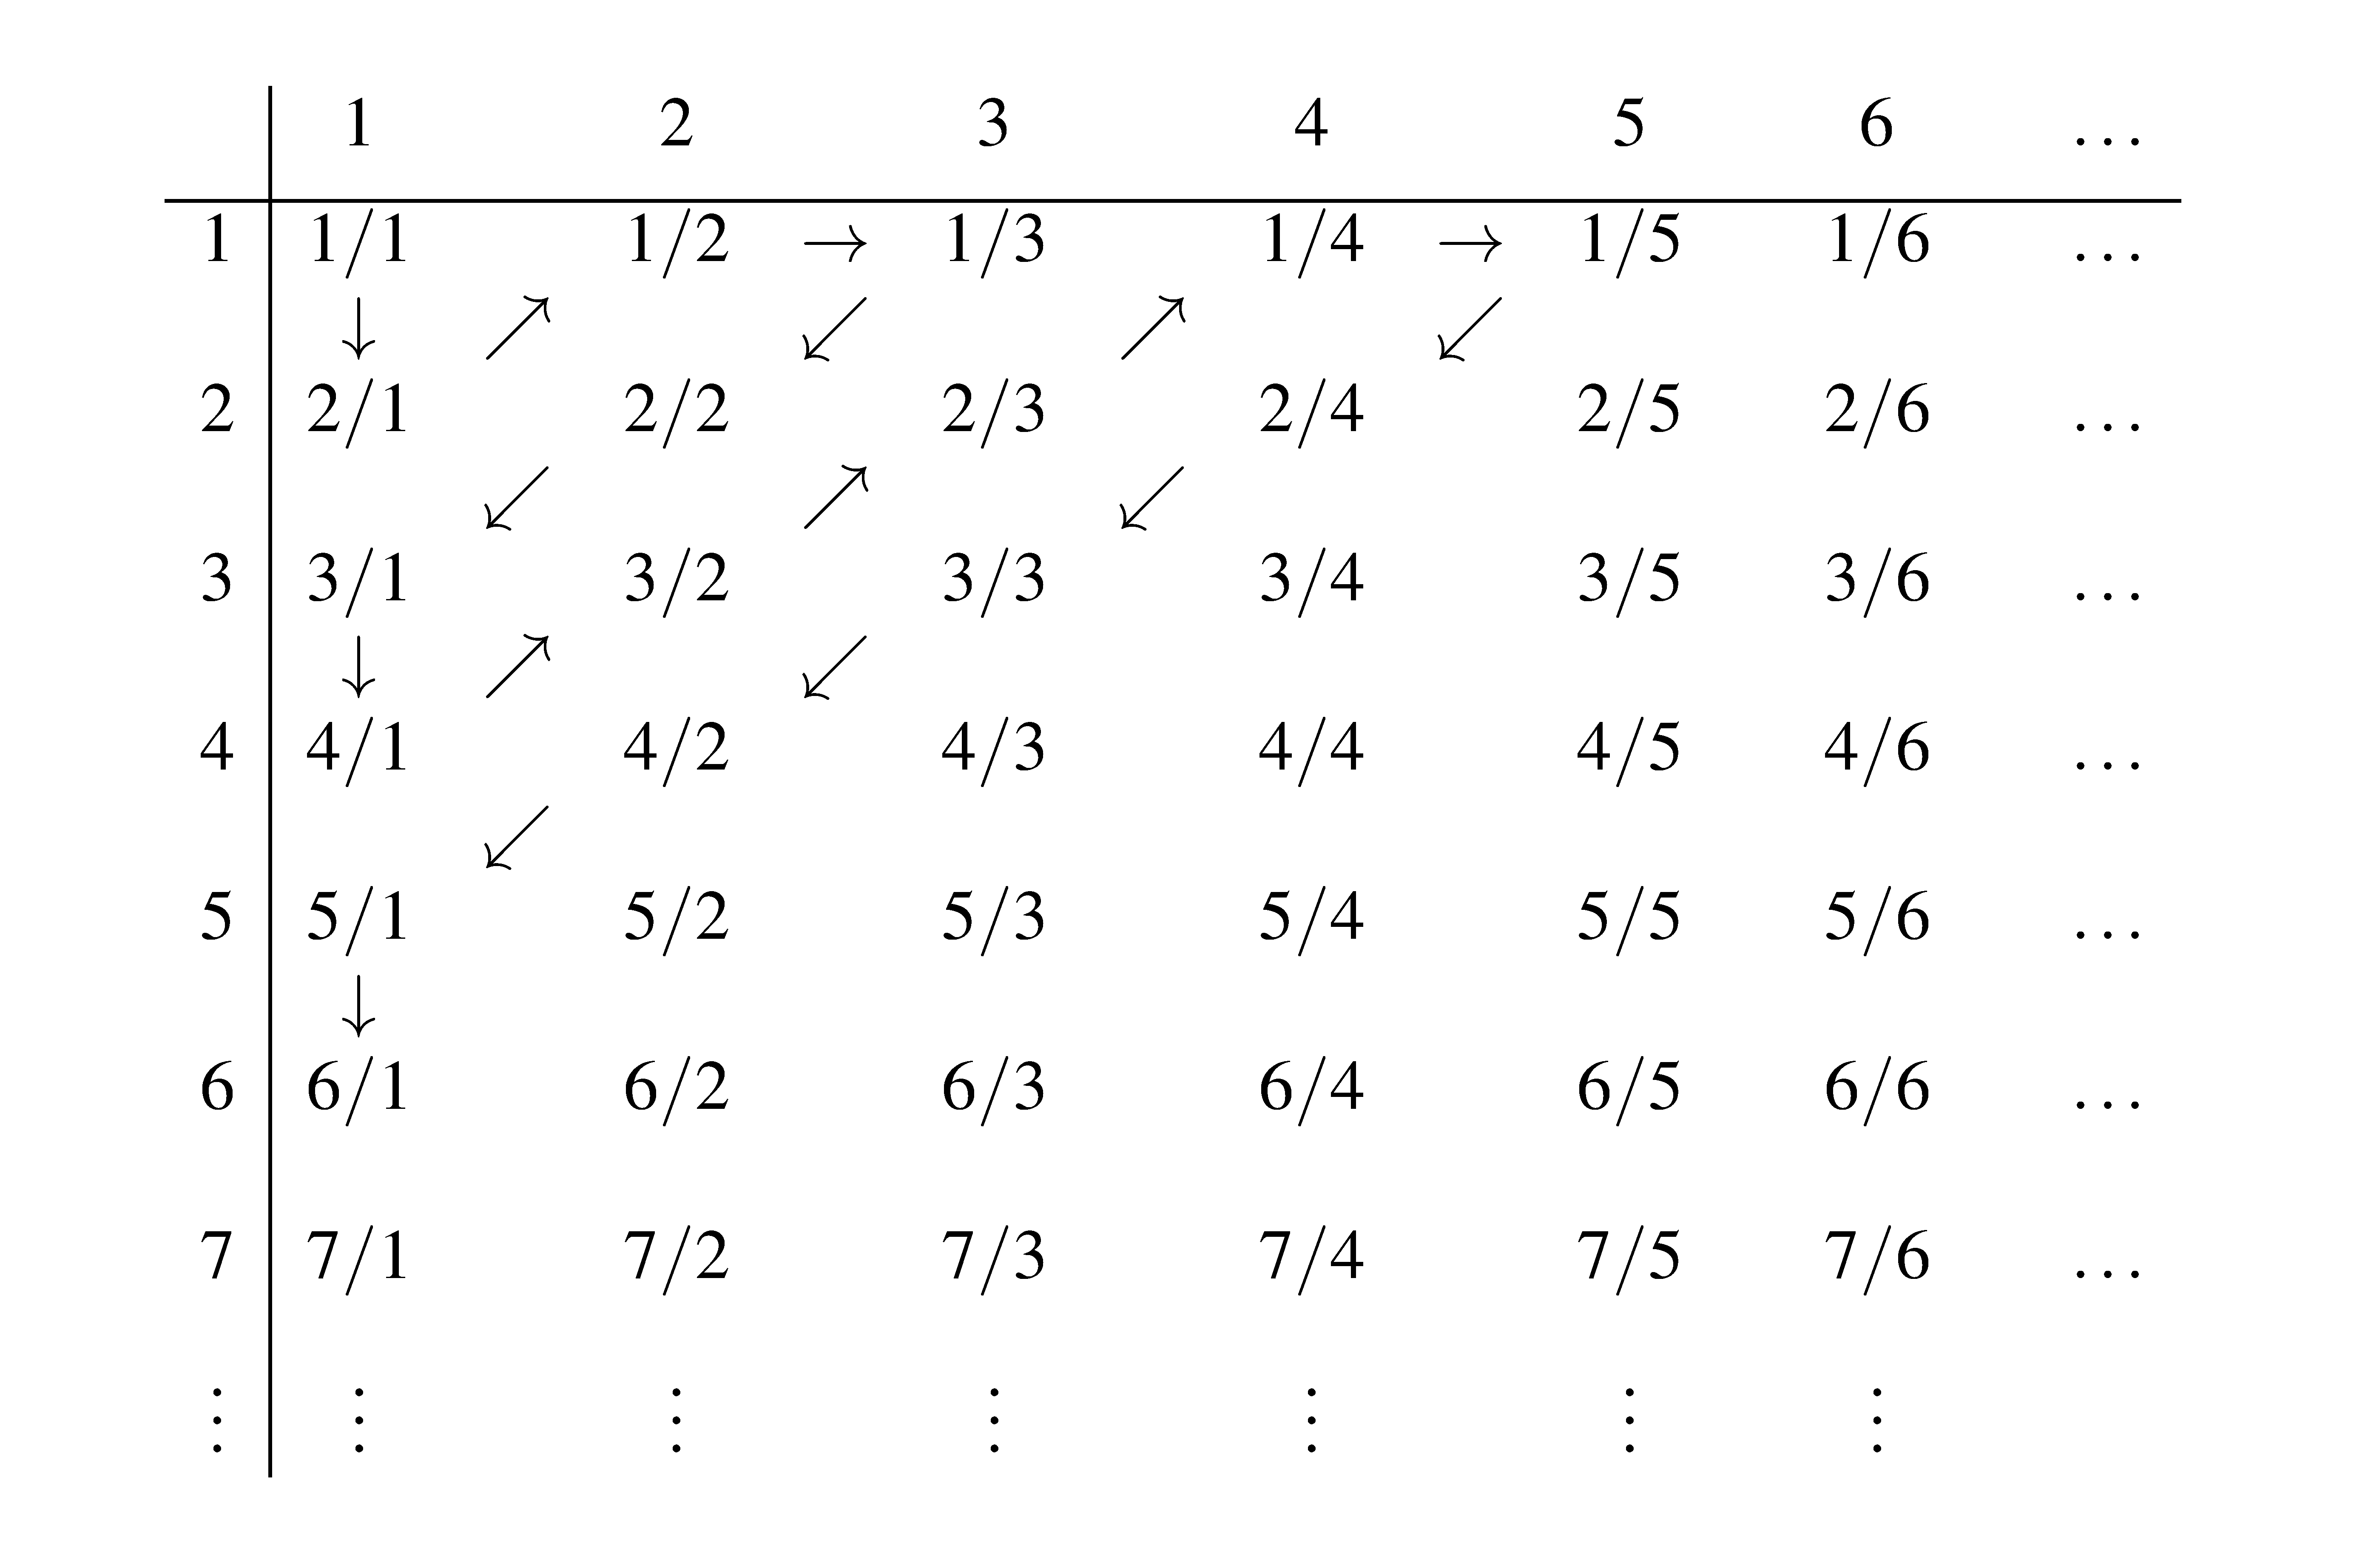
\includegraphics[width=0.8\textwidth]{sup/array}
  

\newcommand{\f}[2]{\small{#1/#2}} 

\newcommand{\ra}{\ensuremath{\rightarrow}} 

\newcommand{\da}{\ensuremath{\downarrow}} 

\newcommand{\nea}{\ensuremath{\nearrow}} 

\newcommand{\swa}{\ensuremath{\swarrow}}
\renewcommand{\arraystretch}{1}
\renewcommand{\tabcolsep}{3pt}

\begin{tabular}{ccccccccccccc}

 \rowcolor{lgray}
 \f{1}{1}	& 		&\f{1}{2}	&\ra  	&\f{1}{3}	& 		&\f{1}{4}	& \ra 	&\f{1}{5}	& 		&\f{1}{6} 	& 	&\ldots\\[0pt]

 \da		&\nea 	&        	&\swa &        		&\nea 	&        	&\swa 	&        	&	 	&        	& 	&	      \\[0pt]

 \rowcolor{lgray}
 \f{2}{1}& &\f{2}{2}& &\f{2}{3}& &\f{2}{4}& &\f{2}{5}& &\f{2}{6}& &\ldots\\[0pt]

		 &  \swa      & & \nea       & & \swa       & &        & &        & &      \\[0pt]

 
\rowcolor{lgray}
 \f{3}{1}& &\f{3}{2}& &\f{3}{3}& &\f{3}{4}& &\f{3}{5}& &\f{3}{6}& &\ldots\\[0pt]


 \da		&\nea &        &\swa &        & &        & &        & &        & &      
 \\[0pt]

 \rowcolor{lgray}
 \f{4}{1}& &\f{4}{2}& &\f{4}{3}& &\f{4}{4}& &\f{4}{5}& &\f{4}{6}& &\ldots\\[0pt]

				& \swa&        & &        & &        & &        & &        & &      \\[0pt]
 
 \rowcolor{lgray}
 \f{5}{1}& &\f{5}{2}& &\f{5}{3}& &\f{5}{4}& &\f{5}{5}& &\f{5}{6}& &\ldots\\[0pt]

				\da	& \nea &        & &        & &        & &        & &        
					& &      \\[0pt]

					
 \rowcolor{lgray}
 \f{6}{1}& &\f{6}{2}& &\f{6}{3}& &\f{6}{4}& &\f{6}{5}& &\f{6}{6}& &\ldots\\[0pt]

		 &        & &        & &        & &        & &        & &      \\[0pt]
 
 \rowcolor{lgray}
 \f{7}{1}& &\f{7}{2}& &\f{7}{3}& &\f{7}{4}& &\f{7}{5}& &\f{7}{6}	& &\ldots\\[0pt]

 
 \vdots &&\vdots  &&\vdots  &&\vdots  &&\vdots  &&\vdots  &&\\


\end{tabular}



\caption{Procedure for enumerating all positive fractions.}
\label{fig:fractions}
 \end{center}
\end{figure}

So fractions are countable: the first is \textfrac{1}{1}, the second is 
\textfrac{2}{1}, the third is \textfrac{1}{2}, etc.  One way of thinking about 
what we are doing is that we are assigning ID numbers to each fraction where 
each ID number is a natural number.  Even though one might feel that there are 
many more fractions than there are natural numbers, we can in fact give each and 
every fraction its own unique ID number without exhausting the pool of ID 
numbers.



\subsection{Countability of sentences}


Suppose \lL[] has infinitely many atomic sentences \p{A_1}, \p{A_2}, \p{A_3}, 
\ldots.  We want to enumerate all sentences of \lL{}. How could we do that? We 
will proceed in stages.

Let us first classify the sentences of \lL{}. We will call our atomic sentences 
class-0 sentences. Class-1 sentences are all class-0 sentences and all complex 
sentences that can be formed out of class-0 sentences by applying a single 
connective once. Class-3 sentences are all class-1 sentences and all complex 
sentences that can be formed out of class-1 sentences by applying a single 
connective once.  More generally:
\begin{description}
 \item[Class-0] sentences are atomic sentences.
 \item[Class-(n+1)] sentences are all class-n sentences plus all sentences that 
  can be formed out of at most two class-n sentences by applying a single 
  connective once.
\end{description}

Notice that any sentence of \lL{} must belong to some class-n (more precisely, 
there is an n such that the sentence belongs to any class-m such that m$\geq$n).
We will now show that for each n, class-n sentences are countable. 

Let's start with class-0 sentences. They are the atomic sentences of \lL{} and 
by the definition of formal languages, class-0 sentences must be countable. So 
class-0 sentences are countable.

What about class-1 sentences? Class-1 sentences are all class-0 sentences and 
all those sentences that can be formed out of class-0 sentences by applying a 
single connective once. Given this definition of class-1 sentences,  a class-1 
sentence must take one of the following forms:
\begin{itemize}
 \item \p{s}
 \item \p{\lnot s}
 \item \p{s\land t}
  \item \p{s\lor t}
 \item \p{s\limplies t}
\end{itemize}
where \p{s} and \p{t} are class-0---i.e., atomic---sentences. So if we have a 
way of walking through each and every pair of class-0 sentences and listing the 
five class-1 sentences that can be formed out of each pair, we have a way of 
enumerating all class-1 sentences. Here is a procedure that will do the job:

\begin{description}
 \item[Enumerating class-1 sentences]
Walk through  the list of fractions and do the following: given the fraction 
\textfrac{n}{m}, list \p{A_n}, \p{\lnot A_n}, \p{A_n\land A_m}, \p{A_n \lor A_m}, 
\p{A_n\limplies A_m} where any \p{A_i} is a class-0 sentence (i.e., an atomic 
sentence).
\end{description}

As we walk through the fractions, we will produce every class-0 sentence as well 
as any complex sentence that can be formed out of class-0 sentences by applying 
a single connective once. So this is a procedure for enumerating all class-1 
sentences in groups of five.

What about class-2 sentences? We can enumerate them, too:

\begin{description}
 \item[Enumerating class-2 sentences]
Walk through  the list of fractions and do the following: given the fraction 
\textfrac{n}{m}, list \p{S_n}, \p{\lnot S_n}, \p{S_n\land S_m}, \p{S_n \lor S_m}, 
\p{S_n\limplies S_m}, where \p{S_1}, \p{S_2}, \ldots are all the class-1 
sentences.
\end{description}

Since we know that class-1 sentences are countable, we know that there is a 
list of class-1 sentences \p{S_1}, \p{S_2}, \ldots that covers all class-1 
sentences and that therefore this procedure will enumerate all class-2 
sentences.  

We could continue in this vein but there are infinitely many classes. We need a 
better way. And there is. The way we enumerate class-1 and class-2 sentences 
shows that for any n we can enumerate class-(n+1) sentences in the following way:

\begin{description}
 \item[Enumerating class-(n+1) sentences]
Walk through  the list of fractions and do the following: given the fraction 
\textfrac{i}{j}, list \p{S_i}, \p{\lnot S_i}, \p{S_i\land S_j}, \p{S_i \lor S_j}, 
\p{S_i\limplies S_j}, where \p{S_1}, \p{S_2}, \ldots are sentences of class-n.
\end{description}

If the sentence of class-n are countable, this procedure will enumerate all 
class-(n+1) sentences. That is, if class-n sentences are countable, so are 
class-(n+1) sentences. We can now see that for any n, class-n sentences are 
countable: class-0 sentences are countable. So class-1 sentences are countable.  
So class-2 sentences are countable. So class-3 sentences are countable. Etc. 


But what about all the sentences of \lL{} taken together? That is, not just the 
sentences of a particular class-n, but all the infinitely many classes taken 
together.  Can we enumerate them? That's easy, too:

\begin{description}
 \item[Enumerating sentences of \lL{}] Walk through the list of fractions and do 
  the following: given the fraction \textfrac{n}{m}, list the m-th sentence of 
  class-n sentences.
\end{description}

For any sentence of \lL{}, it will eventually show up on the list of sentences 
generated in this way. Thus, the sentences of \lL{} are countable even when 
\lL{} has infinitely many atomic sentences. Put another way, you could assign a  
unique natural number as an ID to each and every sentence of \lL{} without 
worrying about exhausting the pool of ID numbers.


\subsection{Things to note about the argument}


Strictly speaking, we have shown more than that the sentences of \lL{} are 
countable. What we have shown is known as recursive enumerativity.  Roughly, 
that means it is possible to write a computer program to generate a list of all 
the sentences of \lL{}.  Not everything that is countable can be enumerated by a 
computer program. For instance, consider a list of all the winning numbers of a 
lottery.  That's countable, but if the lottery organizers know what they are 
doing, it is not possible to write a program that can generate the list of all 
winning numbers. The only way to list up all the winning numbers is by waiting 
for the drawings to take place (otherwise, you could get rich quick by writing a 
program that lists all the winning number, running it faster than the lottery 
numbers are drawn and buying the right tickets).  There is something special and 
interesting about the fact that the sentences of \lL{} are recursively 
enumerable.

The procedure we used for enumerating the sentences of \lL{}  will produce a 
highly redundant list because each class of sentences contains all members of 
the lower-numbered classes. If you don't like redundant lists, you can add the 
instruction `if the sentence has been listed previously, don't list it'.

There are infinitely many ways of enumerating the sentences of \lL{}.  Usually 
sentences are enumerated for a purpose and the method of enumeration used is 
tailored for the purpose.  The way we used here will be useful later for proving 
what is known as completeness of sentential logic               
(Section~\ref{sec:propCompleteness}).   A truly momentous result known as 
G\"odel's Incompleteness Theorem was proven using a different, very clever 
numbering scheme (That theorem concerns a formal language that is more complex 
than \lL{}.)

On a more prosaic level, computers represent sentences as  numbers (by assigning 
a number to each character and stringing them together).  That's a way of 
assigning a unique ID to each distinct sentence. That works, and we don't have 
to worry about running out of numbers to represent sentences. Some numbering 
schemes are easy to reverse in the sense that given an ID number it is 
relatively easy to figure out which sentence it belongs to. Some schemes are 
harder to reverse. Digital encryption works by using schemes that are especially 
difficult to reverse without some extra information (the extra information is 
often called the decryption key). 

What if \lL{} has only finitely many atomic sentences? In that case, each class 
of sentences has only finitely many sentences. But there still are infinitely 
many classes. You can use the same procedure for enumerating sentences of \lL{} 
by adding `if there is no m-th sentence of class-n, skip to the next fraction'.

Suppose there are 100 students and each gets a unique ID number. If we add more 
students to the mix, we will need to get hold of \emph{new} ID numbers to assign 
unique ID numbers to students in the enlarged group. Suppose there are 
infinitely many class-0 sentences. You can assign each sentence a unique ID so 
that each natural number is the ID of some sentence. That is, there are no 
numbers you can add to your pool of ID numbers.  And yet, if you add class-1 
sentences to the mix---there are infinitely many of them---you will be able to 
assign a unique ID to each and every sentence in that combined group of 
sentences by recycling the ID numbers you used for class-0 sentences.  And you 
can do this even if you add infinitely many classes each of which has infinitely 
many sentences. That's a bit mind-boggling. You might suspect that there can be 
no such thing as having so many things you genuinely cannot give them unique IDs, 
but a very simple argument can show that that's not so. Let me close this 
chapter with a discussion of that.



\section{Cantor's Diagonal Argument}\label{sec:diagonalization}

Consider the way we produced the list of interpretations earlier. If there is only one 
atomic sentence, there are two interpretations. As we add an atomic sentence, the number 
of interpretations doubles.  So if there are \p{N} sentences, there are $2^N$ interpretations.   
For instance, if there are 3 atomic sentences, there are $2^3=8$ interpretations.  If 
there are 8 atomic sentences, there are $2^8=256$ interpretations. And so on.  
How many interpretations are there if there  are infinitely many atomic 
sentences?  Well, infinitely many. But is the number of interpretations 
countable? The answer is No.  Here's an argument due to Georg \citet{Cantor1891} 
known as the Diagonal Argument.








Take the way we have been listing interpretations when constructing truth tables.  
Imagine a list of interpretations constructed in that way for infinitely many 
atomic sentences by repeating the procedure infintely many times. We know 
exactly what such a list looks like.  The first row has only T's. The second row 
starts with a single F and is followed by only T's.  The third row starts with a 
T followed by an F and then only T's. The fourth row starts with two F's and 
then only T's.  Etc.  Starting from top of the list, the whole thing will look 
like Figure \ref{fig:inf-tt-table}.


 \begin{center}

\begin{tabular}{cccccccc}

 & \footnotesize{\Circled[outer color=white]{T}}& \footnotesize{\Circled[outer 
color=white]{T}} & \footnotesize{\Circled[outer color=white]{T}} & 
\footnotesize{\Circled[outer color=white]{T}} & \footnotesize{\Circled[outer 
color=white]{T}} & \footnotesize{\Circled[outer color=white]{T}} & \ldots\\ 

 \rowcolor{lgray}
				  & \footnotesize{F} & \footnotesize{T} & \footnotesize{T} & 
 \footnotesize{T} & \footnotesize{T} & \footnotesize{T} & \ldots\\

				  & \footnotesize{T} & \footnotesize{F} & \footnotesize{T} & 
 \footnotesize{T} & \footnotesize{T} & \footnotesize{T} &  \ldots\\


 \rowcolor{lgray}
				  &  \footnotesize{F} & \footnotesize{F} & \footnotesize{T} & 
 \footnotesize{T} & \footnotesize{T} & \footnotesize{T} & \ldots\\

								& \footnotesize{T} & \footnotesize{T} & 
 \footnotesize{F} & \footnotesize{T} & \footnotesize{T} & \footnotesize{T} & 
 \ldots\\


 \rowcolor{lgray}
				  & \footnotesize{F} & \footnotesize{T} & \footnotesize{F} & 
 \footnotesize{T} & \footnotesize{T} & \footnotesize{T} & \ldots\\

				  & \vdots   &\vdots    & \vdots   & \vdots   & \vdots   & 
 \vdots   & \\
\end{tabular}
 \captionof{figure}{interpretations for infinitely many atomic sentences}             
 \label{fig:inf-tt-table}
 \end{center}



It may seem that the table must list all the interpretations. After all, we know exactly 
how to proceed as we increase the number of atomic sentences one by one. At no 
point will the procedure miss an interpretation, so how could the procedure miss 
an interpretation when extending it to infinitely many atomic sentences? And if 
the list of interpretations is complete, clearly the interpretations are 
countable: the first is on the first row, the second is on the second row, etc. 

Matters, however, are not this simple. It is easy to construct an interpretation 
that is not on the list. Here is how. An interpretation can be treated as a just 
a string of T's and F's. Let's construct new interpretation \p{\mathcal N}  in 
the following way:

\begin{itemize}
 \item If the first letter of the first interpretation is a T, the first letter of 
  \p{\mathcal N} is F. If the first letter of the first interpretation is an F, the first 
  letter of \p{\mathcal N} is a T.

 \item If the second letter of the second interpretation is a T, the second letter of 
  \p{\mathcal N} is F. If the second letter of the second interpretation is an F, the 
  second letter of \p{\mathcal N} is a T.

 \item More generally, the n-th letter of \p{\mathcal N} is a T iff. the n-th 
  letter of the n-th interpretation is an F. 

\end{itemize}

The following illustrates the method:
\begin{center}

\begin{tabular}{cccccccc}
 & \footnotesize{\textcircled{T}}& \footnotesize{T} & \footnotesize{T} & 
 \footnotesize{T} & \footnotesize{T} & \footnotesize{T} & \ldots\\ 

 \rowcolor{lgray}
				  & \footnotesize{F} & \footnotesize{\textcircled{T}} & 
 \footnotesize{T} & \footnotesize{T} & \footnotesize{T} & \footnotesize{T} & 
 \ldots\\

				  & \footnotesize{T} & \footnotesize{F} & 
 \footnotesize{\textcircled{T}} & \footnotesize{T} & \footnotesize{T} & 
 \footnotesize{T} &  \ldots\\


 \rowcolor{lgray}
				  &  \footnotesize{F} & \footnotesize{F} & \footnotesize{T} & 
 \footnotesize{\textcircled{T}} & \footnotesize{T} & \footnotesize{T} & \ldots\\

								& \footnotesize{T} & \footnotesize{T} & 
 \footnotesize{F} & \footnotesize{T} & \footnotesize{\textcircled{T}} & 
 \footnotesize{T} & \ldots\\


 \rowcolor{lgray}
				  & \footnotesize{F} & \footnotesize{T} & \footnotesize{F} & 
 \footnotesize{T} & \footnotesize{T} & \footnotesize{\textcircled{T}} & \ldots\\

				  & \vdots   &\vdots    & \vdots   & \vdots   & \vdots   & 
 \vdots   & \\

\hline
 \footnotesize{$\mathcal N$:}	  & \footnotesize{F} & \footnotesize{F} & 
 \footnotesize{F} & \footnotesize{F} & \footnotesize{F} & \footnotesize{F} & 
 \ldots\\

\end{tabular}
\captionof{figure}{Diagonalization}
\end{center}

It shows the top left corner of our list of interpretations. Each row above the 
horizontal line is an infinitely long interpretation.  We construct the 
interpretation \p{\mathcal N} below the horizontal line by taking each circled 
letter and `flipping' it (T to F, F to   T).  \p{\mathcal N} differs from the 
first interpretation because of the first letter, from the second interpretation 
because of the second letter, from the third interpretation because of the third 
letter, etc. \p{\mathcal N} differs from each and every  interpretation on the 
list. That means that \p{\mathcal N} is not on the list.  Thus, the list of 
interpretation is not a complete list.  I hope you can see why the argument is 
called the \emph{Diagonal} Argument. 

The interpretation \p{\mathcal N} we have found is the one  that assigns \emph{F} 
to all atomic sentences. And that cannot be on the list since given the way we 
construct the list of interpretations, that particular interpretation must be 
the last one. But an infinite list cannot have a last line: that's what it is to 
be \emph{infinte}---without end. 

You might think we can handle that problem by simply adding the interpretation we have 
found to the list. Like this:

 \begin{center}

\begin{tabular}{ccccccccc}

	  & \footnotesize{\Circled[outer color=white]{F}} & 
 \footnotesize{\Circled[outer color=white]{F}} & \footnotesize{\Circled[outer 
 color=white]{F}} & \footnotesize{\Circled[outer color=white]{F}} & 
 \footnotesize{\Circled[outer color=white]{F}} & \footnotesize{\Circled[outer 
 color=white]{F}} & \footnotesize{\Circled[outer color=white]{F}}& \ldots\\
 
 \rowcolor{lgray}
				  & \footnotesize{T}& \footnotesize{T} & \footnotesize{T} & 
 \footnotesize{T} & \footnotesize{T} & \footnotesize{T} & \footnotesize{T}  & 
 \ldots\\ 

				  & \footnotesize{F} & \footnotesize{T} & \footnotesize{T} & 
 \footnotesize{T} & \footnotesize{T} & \footnotesize{T} &\footnotesize{T}   
				  &\ldots\\

 \rowcolor{lgray}
				  & \footnotesize{T} & \footnotesize{F} & \footnotesize{T} & 
 \footnotesize{T} & \footnotesize{T} & \footnotesize{T} &\footnotesize{T}    
				  &\ldots\\


				  &  \footnotesize{F} & \footnotesize{F} & \footnotesize{T} & 
 \footnotesize{T} & \footnotesize{T} & \footnotesize{T} &\footnotesize{T}   
				  &\ldots\\

 \rowcolor{lgray}
								& \footnotesize{T} & \footnotesize{T} & 
 \footnotesize{F} & \footnotesize{T} & \footnotesize{T} & \footnotesize{T} 
				  &\footnotesize{T}  & \ldots\\


				  & \footnotesize{F} & \footnotesize{T} & \footnotesize{F} & 
 \footnotesize{T} & \footnotesize{T} & \footnotesize{T} &\footnotesize{T} & 
 \ldots\\

				  & \vdots   &\vdots    & \vdots   & \vdots   & \vdots   & 
 \vdots   & \vdots &  \\
\end{tabular}
\captionof{figure}{list of interpretations with missing interpretation added}             
\end{center}

But this won't do. We can construct a interpretation that is not on this list: 

\begin{center}
\begin{tabular}{ccccccccc}

	  & \footnotesize{\textcircled{F}} & \footnotesize{F} & \footnotesize{F} & 
 \footnotesize{F} & \footnotesize{F} & \footnotesize{F} & \footnotesize{F} 
				  &\ldots\\
 
 \rowcolor{lgray}
				  
				  & \footnotesize{T}& \footnotesize{\textcircled{T}} & 
 \footnotesize{T} & \footnotesize{T} & \footnotesize{T} & \footnotesize{T} & 
 \footnotesize{T} & \ldots\\
				  
				  & \footnotesize{F} & \footnotesize{T} & 
 \footnotesize{\textcircled{T}} & \footnotesize{T} & \footnotesize{T} & 
 \footnotesize{T} & \footnotesize{T} & \ldots\\

 \rowcolor{lgray}
				  & \footnotesize{T} & \footnotesize{F} & \footnotesize{T} & 
 \footnotesize{\textcircled{T}} & \footnotesize{T} & \footnotesize{T} &  
 \footnotesize{T} & \ldots\\


				  &  \footnotesize{F} & \footnotesize{F} & \footnotesize{T} & 
 \footnotesize{T} & \footnotesize{\textcircled{T}} & \footnotesize{T} & 
 \footnotesize{T} & \ldots\\

 \rowcolor{lgray}
								& \footnotesize{T} & \footnotesize{T} & 
 \footnotesize{F} & \footnotesize{T} & \footnotesize{T} & 
 \footnotesize{\textcircled{T}} &\footnotesize{T} &  \ldots\\


				  & \footnotesize{F} & \footnotesize{T} & \footnotesize{F} & 
 \footnotesize{T} & \footnotesize{T} & \footnotesize{T} & 
 \footnotesize{\textcircled{T}} & \ldots\\

				  & \vdots   &\vdots    & \vdots   & \vdots   & \vdots   & 
 \vdots   & \vdots   &\\
\hline
 \footnotesize{$\mathcal N$:}	  & \footnotesize{T} & \footnotesize{F} & 
 \footnotesize{F} & \footnotesize{F} & \footnotesize{F} & \footnotesize{F} & 
 \footnotesize{F} &
 \ldots\\
\end{tabular}
\captionof{figure}{Finding another missing interpretation}

\end{center}


The point is completely general. It is not just that our particular way of 
generating the list of interpretations fails when dealing with infinitely many 
atomic sentences. Given any list of interpretations for infinitely many atomic 
sentences, we can find an interpretation that is not on the list.  Here is an 
illustration to see that:

\begin{center}

\begin{tabular}{cccccccc}

 & \textcircled{\footnotesize{T}} & \footnotesize{F} & \footnotesize{T} & 
 \footnotesize{T} & \footnotesize{F} & \footnotesize{T} & \ldots\\ 

 \rowcolor{lgray}
				  & \footnotesize{F} & \textcircled{\footnotesize{T}} & 
 \footnotesize{F} & \footnotesize{F} & \footnotesize{T} & \footnotesize{T} & 
 \ldots\\

				  & \footnotesize{T} & \footnotesize{T} & 
 \textcircled{\footnotesize{F}} & \footnotesize{T} & \footnotesize{T} & 
 \footnotesize{T} &  \ldots\\


 \rowcolor{lgray}
				  &  \footnotesize{F} & \footnotesize{F} & \footnotesize{F} & 
 \textcircled{\footnotesize{T}} & \footnotesize{F} & \footnotesize{T} & \ldots\\

								& \footnotesize{F} & \footnotesize{F} & 
 \footnotesize{F} & \footnotesize{T} & \textcircled{\footnotesize{F}} & 
 \footnotesize{F} & \ldots\\


 \rowcolor{lgray}
				  & \footnotesize{T} & \footnotesize{T} & \footnotesize{T} & 
 \footnotesize{T} & \footnotesize{F} & \textcircled{\footnotesize{T}} & \ldots\\

				  & \vdots   &\vdots    & \vdots   & \vdots   & \vdots   & 
 \vdots   & \\
\hline
 \footnotesize{$\mathcal N$:}	  & \footnotesize{F} & \footnotesize{F} & 
 \footnotesize{T} & \footnotesize{F} & \footnotesize{T} & \footnotesize{F} & 
 \ldots\\
\end{tabular}

\end{center}

That means, the very idea of a complete list of interpretations when dealing with 
infinitely many atomic sentence is incoherent.  That is what the Diagonal 
Argument shows.  Given infinitely many atomic sentences, there are more interpretations 
than there are natural numbers.  We say that the set of interpretations has higher 
\emph{cardinality} than the natural numbers.

We now know that there really are more interpretations than there are atomic 
sentences---that's even true if the number of atomic sentences is infinite as we 
have just shown. What about the number of truth conditions? 

A truth condition of a sentence  specifies for each interpretation whether or not the 
sentence is true in that interpretation.  That means that if \p{\mathtt{m}} is the 
number of interpretations, the number of possible truth conditions is \p{2^\mathtt{m}}.  
For instance, if there are 8 atomic sentences, there are 256 interpretations  and $2^{256}
\approx 1.1\times 10^{77}$ possible truth conditions.  For comparison, our 
planet Earth is estimated to contain about $10^{50}$ atoms.\footnote{\url{https:
//www.fnal.gov/pub/science/inquiring/questions/atoms.html}}
With just one more atomic sentence---9 of them---there are about $2^{512}\approx 
1.3\times 10^{154}$ possible truth conditions for a sentence. That vastly---and 
that's putting it very mildly---exceeds the estimated number of atoms in the 
observable universe which is around $10^{80}$ atoms.\footnote{\url{https:
//en.wikipedia.org/wiki/Observable_universe}} This gives you a glimpse of the 
expressive capacities of natural languages: they can surely say more than what 
we can with just 9 atomic sentences in \lL{}. 

These considerations show that the number of truth conditions is larger than the 
number of interpretations in case the number of atomic sentences is finite.  And we can 
prove that this is so even if there are infinitely many atomic sentences.

The proof proceeds via a slight reformulation of the Diagonal Argument.  Notice 
that the question whether or not there are countably many interpretations is the 
same as the question whether or not  it is possible to pair atomic sentences 
with interpretations without residue on either side. An interpretation can be 
understood as a subset of atomic sentences: each interpretation contains those 
atomic sentences that are true in that interpretation. So the question is 
whether or not the set of atomic sentences can be paired, without residue on 
either side,  with sets of atomic sentences---these latter are the subsets of 
the set of atomic sentences.  Take any set \p{\mathcal S} and consider a pairing 
of its members with subsets of \p{\mathcal S}. Could such a pairing be 
one-to-one without residue? The answer is no.  We can construct a  new subset 
\p{\mathcal N} in the following way: for any member \p{e} of \p{\mathcal S}, 
\p{e} is in \p{\mathcal N} iff.  \p{e} is not in the subset of \p{\mathcal S} 
paired with it.  \p{\mathcal N} is not paired with any member of \p{\mathcal S} 
since for any member \p{e} of \p{\mathcal S}, \p{\mathcal N} differs from the 
subset of \p{\mathcal S} paired with \p{e}. This shows that the cardinality of 
the set of all the subsets of \p{\mathcal S}---a.k.a. the \emph{power set} of 
\p{\mathcal S}---must be larger than the cardinality of \p{\mathcal S}.  This is 
known as Cantor's Theorem. 

The argument just given can be given for any set and its power set: thus, as we 
have already seen, the set of interpretations has higher cardinality than the 
set of all atomic sentences. Now, a truth condition is a set of interpretations: 
the set of all the interpretations in which a sentence is true.  So the 
cardinality of truth conditions is higher than the cardinality of 
interpretations. And the set of all the subsets of truth conditions has even 
higher cardinality, and so on.   This opens up a realm of mathematical entities 
that David Hilbert called Cantor's paradise  \citeyearpar{hilbert1926}.




